\chapter{Measurement of PDP}
To find the delay spread and ultimately the coherence bandwidth a \gls{PDP} measurement is necessary. 
\section{Setup}
The PNA is preforming a frequency sweep and using an inverse transformation to convert from the frequency to the time domain.
The PDP profile is measured at 20 different positions in the measuring area in \autoref{meas_area} and averaged over. 

\begin{table}[H]
\centering
\begin{tabular}{|l|l|l|l|}
\hline
\textbf{Name}					& \textbf{Symbol} & \textbf{Value} 	& \textbf{Reference} 		\\ \hline
Center Frequency                & $f_c$       	& 5Ghz              & \autoref{equipment}		\\ \hline
Span 							& $f_{Span}$ 	& 1GHz 				& \autoref{sec:setup_parameter} \\ \hline
Average SNR	                   	& SNR          	& 67dB            	& appendix  \ref{app:SNR} 	\\ \hline
Antenna diversity               & $A_{div}$   	& 1x3    			& \autoref{equipment} 		\\ \hline
Intermediate frequency bandwidth & $IF_{BW}$    & 500Hz   			& \autoref{sec:setup_parameter} \\ \hline
Cable loss 						& $L_{C}$     	& 7dB         		& \autoref{equipment} 		\\ \hline
Number of points per sweep 		& $N_{sweep}$ 	& 801				& \autoref{sec:coherence_bandwidth} \\ \hline
Transmit power 					& $P_{TX}$ 		& 17dBm				& \autoref{equipment} 		\\ \hline
Antenna Gain 					& $G_{ANT}$ 	& 12dBi 			& \autoref{equipment} \\ \hline
Sweep time 						& $T_{sweep}$ 	& 1448msec			& \autoref{sec:setup_parameter} \\ \hline
\end{tabular}
\caption{VNA settings during PDP measurements}
\label{pdp_specs}
\end{table}

%\section{Results}
%
%\begin{figure}[H]
%\centering
%% This file was created by matlab2tikz.
%
%The latest updates can be retrieved from
%  http://www.mathworks.com/matlabcentral/fileexchange/22022-matlab2tikz-matlab2tikz
%where you can also make suggestions and rate matlab2tikz.
%
\definecolor{mycolor1}{rgb}{0.00000,0.44700,0.74100}%
%
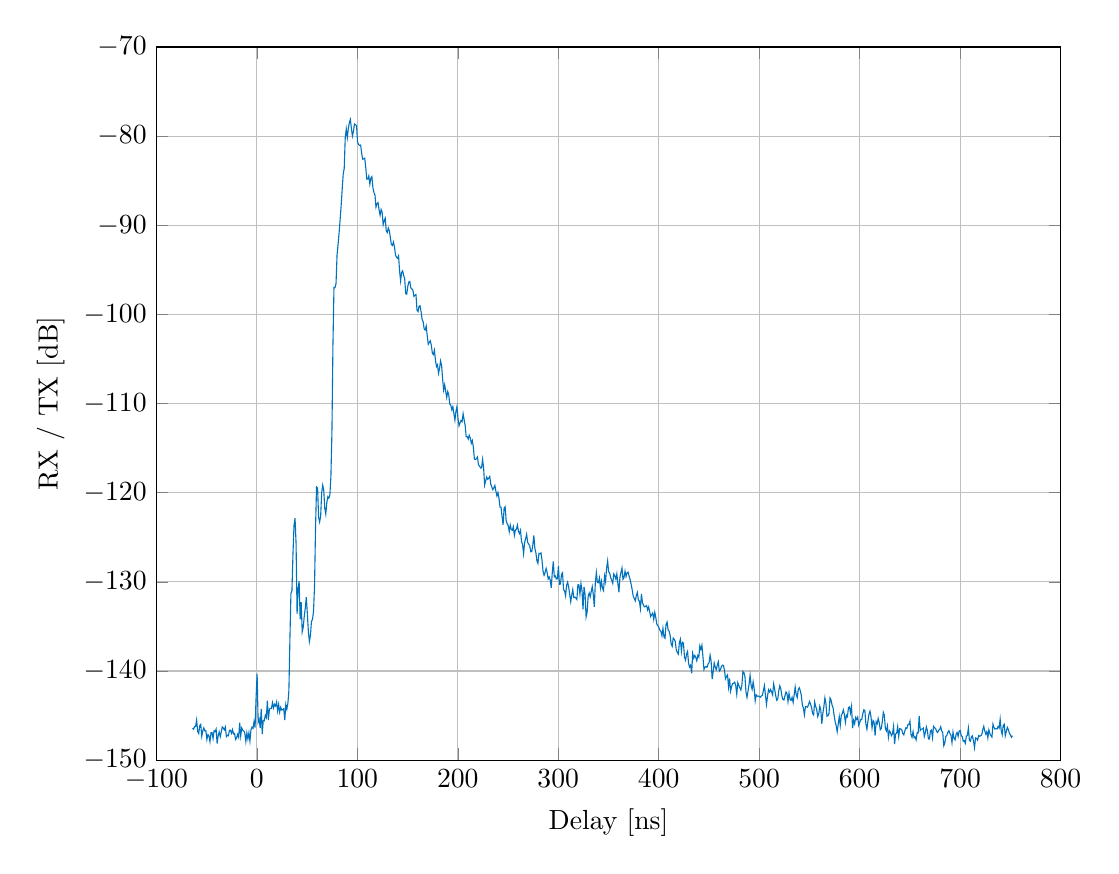
\begin{tikzpicture}

\begin{axis}[%
width=4.521in,
height=3.566in,
at={(0.758in,0.481in)},
scale only axis,
xmin=-100,
xmax=800,
xlabel={Delay [ns]},
xmajorgrids,
ymin=-150,
ymax=-70,
ylabel={RX / TX [dB]},
ymajorgrids,
axis background/.style={fill=white}
]
\addplot [color=mycolor1,solid,forget plot]
  table[row sep=crcr]{%
-64.0081	-146.390936907367\\
-62.98795075	-146.522206789345\\
-61.9678015	-146.234394862441\\
-60.94765225	-146.217471135383\\
-59.927503	-145.494010526581\\
-58.90735375	-146.793791781355\\
-57.8872045	-147.026644758051\\
-56.86705525	-146.14096744394\\
-55.846906	-145.990224741517\\
-54.82675675	-147.321006272119\\
-53.8066075	-146.732179088988\\
-52.78645825	-146.382942629889\\
-51.766309	-146.717495740693\\
-50.74615975	-146.694660864063\\
-49.7260105	-147.672951224379\\
-48.70586125	-147.135336280423\\
-47.685712	-147.271651087558\\
-46.66556275	-147.931693863493\\
-45.6454135	-146.929252002212\\
-44.62526425	-146.919933701446\\
-43.605115	-147.573417622976\\
-42.58496575	-146.708030428174\\
-41.5648165	-146.813874307169\\
-40.54466725	-146.52195276916\\
-39.524518	-148.147163630164\\
-38.50436875	-147.259684655576\\
-37.4842195	-146.831561472582\\
-36.46407025	-147.371826406778\\
-35.443921	-146.84379479896\\
-34.42377175	-146.271104298596\\
-33.4036225	-146.399672703352\\
-32.38347325	-146.604181746801\\
-31.363324	-146.287801447648\\
-30.34317475	-147.365823545641\\
-29.3230255	-147.202852727994\\
-28.30287625	-147.2679546519\\
-27.282727	-146.650640379146\\
-26.26257775	-146.650087696784\\
-25.2424285	-146.988979549387\\
-24.22227925	-146.578365483772\\
-23.20213	-147.066265025169\\
-22.18198075	-147.009495473774\\
-21.1618315	-147.676031204919\\
-20.14168225	-147.495831026144\\
-19.121533	-147.106189222467\\
-18.10138375	-147.447056715858\\
-17.0812345	-145.800012934975\\
-16.06108525	-147.282062209807\\
-15.040936	-146.394968227941\\
-14.02078675	-146.658602971217\\
-13.0006375	-146.722084344881\\
-11.98048825	-146.975003099505\\
-10.960339	-147.905520578456\\
-9.94018975	-146.950000239202\\
-8.9200405	-147.621650019954\\
-7.89989125	-146.931576902086\\
-6.879742	-147.857992222206\\
-5.85959275	-146.615117383128\\
-4.8394435	-146.30002077309\\
-3.81929425	-146.440453941961\\
-2.799145	-145.654590094023\\
-1.77899575	-146.350459054578\\
-0.7588465	-142.991702330429\\
0.26130274999999	-140.287661504469\\
1.281452	-145.74554967677\\
2.30160125	-145.400824587122\\
3.3217505	-146.387869967993\\
4.34189975	-144.264846390469\\
5.362049	-147.091368485118\\
6.38219825	-145.54095937231\\
7.4023475	-145.593518136572\\
8.42249675	-144.969101885836\\
9.442646	-145.21881180453\\
10.46279525	-143.336984323649\\
11.4829445	-145.495138156178\\
12.50309375	-144.27817787064\\
13.523243	-144.195994713307\\
14.54339225	-144.205672266574\\
15.5635415	-143.550617080165\\
16.58369075	-144.15096934783\\
17.60384	-143.738744919093\\
18.62398925	-143.923571563781\\
19.6441385	-143.484119458503\\
20.66428775	-144.483957973225\\
21.684437	-143.765504843054\\
22.70458625	-144.624934478052\\
23.7247355	-144.079861303907\\
24.74488475	-144.384607963755\\
25.765034	-144.323150549694\\
26.78518325	-144.233981783546\\
27.8053325	-145.514378407545\\
28.82548175	-143.766265124735\\
29.845631	-144.283515355213\\
30.86578025	-143.651471554773\\
31.8859295	-142.224365874807\\
32.90607875	-136.430187128307\\
33.926228	-131.293957827028\\
34.94637725	-130.984951243438\\
35.9665265	-126.838881527305\\
36.98667575	-123.690935728614\\
38.006825	-122.851630081212\\
39.02697425	-125.659766207352\\
40.0471235	-133.581888339209\\
41.06727275	-130.84607166096\\
42.087422	-129.914147893878\\
43.10757125	-134.20948367528\\
44.1277205	-132.285616979446\\
45.14786975	-135.61229345567\\
46.168019	-135.08578969843\\
47.18816825	-133.853332899614\\
48.2083175	-132.947949990643\\
49.22846675	-131.719879082341\\
50.248616	-133.522409069976\\
51.26876525	-135.549169235793\\
52.2889145	-136.703385528065\\
53.30906375	-136.051241823431\\
54.329213	-134.468208677796\\
55.34936225	-134.209551890707\\
56.3695115	-133.384219989126\\
57.38966075	-130.559417746117\\
58.40981	-123.969966565435\\
59.42995925	-119.345161486758\\
60.4501085	-119.460752970653\\
61.47025775	-122.727031724827\\
62.490407	-123.288599174109\\
63.51055625	-122.630356500872\\
64.5307055	-120.006806963767\\
65.55085475	-119.150458153366\\
66.571004	-119.695291131324\\
67.59115325	-121.742603658648\\
68.6113025	-122.39592103285\\
69.63145175	-121.104378282915\\
70.651601	-120.453401156301\\
71.67175025	-120.607870850219\\
72.6918995	-120.243145121928\\
73.71204875	-118.198101687992\\
74.732198	-113.19105772346\\
75.75234725	-103.353196186593\\
76.7724965	-96.973628166922\\
77.79264575	-96.9840621626918\\
78.812795	-96.5534485100018\\
79.83294425	-93.3201233746722\\
80.8530935	-92.1479444744006\\
81.87324275	-90.8398171427834\\
82.893392	-89.3649746277812\\
83.91354125	-87.80160657656\\
84.9336905	-85.9745194706136\\
85.95383975	-84.2804764293159\\
86.973989	-83.6153574216526\\
87.99413825	-80.1508794906148\\
89.0142875	-79.2065154106393\\
90.03443675	-80.1637324791761\\
91.054586	-79.1447711014508\\
92.07473525	-78.4964709729663\\
93.0948845	-78.1312655560683\\
94.11503375	-79.1369868635284\\
95.135183	-79.9929658314357\\
96.15533225	-79.4646774133908\\
97.1754815	-78.6370940787417\\
98.19563075	-78.7343100309387\\
99.21578	-78.802281007752\\
100.23592925	-80.6793468103798\\
101.2560785	-80.9341468242016\\
102.27622775	-81.0368982241446\\
103.296377	-80.9999922784009\\
104.31652625	-81.9102627878192\\
105.3366755	-82.588610005646\\
106.35682475	-82.5574740341278\\
107.376974	-82.4750517681178\\
108.39712325	-83.5113000879856\\
109.4172725	-84.8311640652247\\
110.43742175	-84.8310875395166\\
111.457571	-84.4571909216726\\
112.47772025	-85.3821380185332\\
113.4978695	-84.7074235719719\\
114.51801875	-84.5441361644513\\
115.538168	-85.7896821257376\\
116.55831725	-86.3400185365793\\
117.5784665	-86.6108258243536\\
118.59861575	-87.9641662144094\\
119.618765	-87.5657335943351\\
120.63891425	-87.4622187610488\\
121.6590635	-88.2857779980279\\
122.67921275	-88.8807585944155\\
123.699362	-88.2249552108159\\
124.71951125	-88.5335955152146\\
125.7396605	-89.9418082744346\\
126.75980975	-89.5028278606095\\
127.779959	-89.2012057473166\\
128.80010825	-90.6140964571652\\
129.8202575	-90.8134640769787\\
130.84040675	-90.2981523441647\\
131.860556	-90.6086360430937\\
132.88070525	-91.3780382429659\\
133.9008545	-92.168271407917\\
134.92100375	-92.2768167008932\\
135.941153	-91.8704052920004\\
136.96130225	-92.4149704826686\\
137.9814515	-93.3110688933367\\
139.00160075	-93.597572094843\\
140.02175	-93.6934694689724\\
141.04189925	-93.4275577780104\\
142.0620485	-95.1019980563616\\
143.08219775	-96.2318511839153\\
144.102347	-95.2849551035595\\
145.12249625	-95.1180475933523\\
146.1426455	-95.6253444230186\\
147.16279475	-96.0192867198322\\
148.182944	-97.6734994736086\\
149.20309325	-97.7248308916071\\
150.2232425	-96.8756120980724\\
151.24339175	-96.3729974113825\\
152.263541	-96.312990742548\\
153.28369025	-97.0344210181446\\
154.3038395	-97.1348395165659\\
155.32398875	-97.2733029252773\\
156.344138	-97.9783354763241\\
157.36428725	-97.8458609616249\\
158.3844365	-97.7917804785588\\
159.40458575	-99.5104457897485\\
160.424735	-99.6884438183996\\
161.44488425	-99.0758289623803\\
162.4650335	-99.0359176741892\\
163.48518275	-99.7229428013719\\
164.505332	-100.557552963213\\
165.52548125	-100.811336408285\\
166.5456305	-101.626514622478\\
167.56577975	-101.746076393876\\
168.585929	-101.307778880856\\
169.60607825	-102.415896004505\\
170.6262275	-103.348302478909\\
171.64637675	-103.129992064089\\
172.666526	-102.966149799845\\
173.68667525	-103.476935397701\\
174.7068245	-104.357354489255\\
175.72697375	-104.508023380276\\
176.747123	-104.020375062909\\
177.76727225	-105.104997113919\\
178.7874215	-105.856517452619\\
179.80757075	-105.652374978426\\
180.82772	-106.617540372024\\
181.84786925	-106.073288002895\\
182.8680185	-105.219230938597\\
183.88816775	-105.716638864355\\
184.908317	-107.221426699938\\
185.92846625	-108.487291201653\\
186.9486155	-107.890044036143\\
187.96876475	-108.629086263301\\
188.988914	-109.331402838048\\
190.00906325	-108.648596697153\\
191.0292125	-109.035949988523\\
192.04936175	-110.07017881784\\
193.069511	-110.198228646362\\
194.08966025	-110.703638139043\\
195.1098095	-110.351198760076\\
196.12995875	-111.105672136851\\
197.150108	-111.865819436362\\
198.17025725	-110.900918545312\\
199.1904065	-110.333041859218\\
200.21055575	-111.641929559713\\
201.230705	-112.492300130928\\
202.25085425	-112.182196292478\\
203.2710035	-111.89704101956\\
204.29115275	-112.029173572619\\
205.311302	-111.133471262737\\
206.33145125	-111.842788167793\\
207.3516005	-112.452471722907\\
208.37174975	-113.719427025113\\
209.391899	-113.705931339011\\
210.41204825	-113.984992290041\\
211.4321975	-113.555594114154\\
212.45234675	-113.869557979526\\
213.472496	-114.46110963798\\
214.49264525	-114.153434738747\\
215.5127945	-114.878951203337\\
216.53294375	-116.233725643816\\
217.553093	-116.269810392383\\
218.57324225	-116.192028617416\\
219.5933915	-116.005128173466\\
220.61354075	-116.872107806928\\
221.63369	-116.985702557162\\
222.65383925	-117.238882437419\\
223.6739885	-117.217196815427\\
224.69413775	-116.260142613752\\
225.714287	-117.208540575466\\
226.73443625	-119.14553492702\\
227.7545855	-118.648432372986\\
228.77473475	-118.238823671159\\
229.794884	-118.503560634091\\
230.81503325	-118.359051831142\\
231.8351825	-118.176072018116\\
232.85533175	-119.064047169008\\
233.875481	-119.330739657656\\
234.89563025	-119.668435044597\\
235.9157795	-119.456958287068\\
236.93592875	-119.192267605092\\
237.956078	-119.833565556744\\
238.97622725	-120.364983157535\\
239.9963765	-119.989667616113\\
241.01652575	-120.617959874006\\
242.036675	-121.621104439293\\
243.05682425	-121.631648789222\\
244.0769735	-122.694568279728\\
245.09712275	-123.591671654888\\
246.117272	-121.738308324729\\
247.13742125	-121.576655426553\\
248.1575705	-123.107223605154\\
249.17771975	-123.498362791703\\
250.197869	-123.688554548929\\
251.21801825	-124.381624215972\\
252.2381675	-123.6118056964\\
253.25831675	-124.125500667037\\
254.278466	-124.216358721955\\
255.29861525	-123.81546048043\\
256.3187645	-124.791275139552\\
257.33891375	-124.192611324934\\
258.359063	-124.093222212308\\
259.37921225	-123.624819848716\\
260.3993615	-124.312620354961\\
261.41951075	-124.58519285396\\
262.43966	-124.218579024858\\
263.45980925	-125.467207640361\\
264.4799585	-125.799272091152\\
265.50010775	-126.848084457436\\
266.520257	-125.625251351364\\
267.54040625	-125.156474762186\\
268.5605555	-124.66072290103\\
269.58070475	-125.582920152478\\
270.600854	-125.766294888247\\
271.62100325	-125.964066473052\\
272.6411525	-126.627877342378\\
273.66130175	-126.609190802353\\
274.681451	-125.858659355476\\
275.70160025	-124.789095840216\\
276.7217495	-126.235202646306\\
277.74189875	-126.730345399093\\
278.762048	-127.642984426081\\
279.78219725	-127.927539611525\\
280.8023465	-126.813581249516\\
281.82249575	-126.853816152365\\
282.842645	-126.75699247303\\
283.86279425	-127.585495699591\\
284.8829435	-128.815108415663\\
285.90309275	-129.265255502736\\
286.923242	-128.952717048244\\
287.94339125	-128.501638338741\\
288.9635405	-128.958216858712\\
289.98368975	-129.675608628374\\
291.003839	-129.453899484603\\
292.02398825	-129.796329979709\\
293.0441375	-130.664398535089\\
294.06428675	-128.965188586771\\
295.084436	-127.706288454121\\
296.10458525	-129.438028549214\\
297.1247345	-129.334004896225\\
298.14488375	-129.679795199434\\
299.165033	-129.65508608849\\
300.18518225	-128.239887367559\\
301.2053315	-130.273638493608\\
302.22548075	-130.25305438591\\
303.24563	-129.166744275175\\
304.26577925	-128.984894307522\\
305.2859285	-130.892489052758\\
306.30607775	-130.979945923887\\
307.326227	-131.565242258\\
308.34637625	-130.371872186491\\
309.3665255	-130.043538358791\\
310.38667475	-130.612368059271\\
311.406824	-131.400198010427\\
312.42697325	-132.229849164517\\
313.4471225	-131.496230622388\\
314.46727175	-130.874585770412\\
315.487421	-131.755466026111\\
316.50757025	-131.709321074442\\
317.5277195	-131.817468369552\\
318.54786875	-131.979085125205\\
319.568018	-130.328559804197\\
320.58816725	-130.338898690601\\
321.6083165	-131.381703143682\\
322.62846575	-130.197106055433\\
323.648615	-130.983217237528\\
324.66876425	-133.084705527866\\
325.6889135	-130.559637898386\\
326.70906275	-131.407937776825\\
327.729212	-133.930234993392\\
328.74936125	-133.417785703941\\
329.7695105	-131.629672937797\\
330.78965975	-131.255234527819\\
331.809809	-131.690615913911\\
332.82995825	-131.093605761198\\
333.8501075	-130.535976138543\\
334.87025675	-131.389350932582\\
335.890406	-132.796979684999\\
336.91055525	-130.13092212913\\
337.9307045	-128.962102329169\\
338.95085375	-130.070447420258\\
339.971003	-130.095422953925\\
340.99115225	-129.563016936726\\
342.0113015	-130.690159262601\\
343.03145075	-129.935290027113\\
344.0516	-130.735882404909\\
345.07174925	-130.985051752043\\
346.0918985	-129.350845772864\\
347.11204775	-129.97873360928\\
348.132197	-128.448899136485\\
349.15234625	-127.660577599463\\
350.1724955	-128.873956613784\\
351.19264475	-129.005866512673\\
352.212794	-129.527544244425\\
353.23294325	-129.839690778421\\
354.2530925	-130.184326533327\\
355.27324175	-129.109543518331\\
356.293391	-129.31128561058\\
357.31354025	-129.689353737503\\
358.3336895	-129.103308225066\\
359.35383875	-130.178935532454\\
360.373988	-131.163467127065\\
361.39413725	-129.521654665028\\
362.4142865	-128.940511638739\\
363.43443575	-128.447285567191\\
364.454585	-129.713012784386\\
365.47473425	-129.518769045178\\
366.4948835	-128.799327798275\\
367.51503275	-129.402062839978\\
368.535182	-128.987088578526\\
369.55533125	-128.907887297983\\
370.5754805	-129.380839706413\\
371.59562975	-129.774920236731\\
372.615779	-130.30453550232\\
373.63592825	-130.909261209065\\
374.6560775	-131.600448383648\\
375.67622675	-131.859588616811\\
376.696376	-132.131859539943\\
377.71652525	-131.557150554737\\
378.7366745	-131.184585558496\\
379.75682375	-132.03436552768\\
380.776973	-132.173369200205\\
381.79712225	-133.011145255106\\
382.8172715	-131.353921538418\\
383.83742075	-132.349592678116\\
384.85757	-132.628342878376\\
385.87771925	-132.799561684648\\
386.8978685	-132.763828620732\\
387.91801775	-132.670211776627\\
388.938167	-133.143927428906\\
389.95831625	-132.815117049744\\
390.9784655	-133.332420855578\\
391.99861475	-133.892449604728\\
393.018764	-133.693598551276\\
394.03891325	-133.501464022305\\
395.0590625	-134.211386226115\\
396.07921175	-133.424702950937\\
397.099361	-133.991511647191\\
398.11951025	-134.73967852302\\
399.1396595	-134.921176674954\\
400.15980875	-135.112193262897\\
401.179958	-135.421444039022\\
402.20010725	-135.563083620552\\
403.2202565	-136.048119547894\\
404.24040575	-135.219575462632\\
405.260555	-136.183641898286\\
406.28070425	-136.319428768735\\
407.3008535	-134.786969760322\\
408.32100275	-134.513381597464\\
409.341152	-135.362855762725\\
410.36130125	-135.541536036641\\
411.3814505	-136.009246773412\\
412.40159975	-136.976105298441\\
413.421749	-137.227215006469\\
414.44189825	-136.29950642971\\
415.4620475	-136.458443648932\\
416.48219675	-136.693165999973\\
417.502346	-137.621692419966\\
418.52249525	-137.928051238765\\
419.5426445	-138.104803743659\\
420.56279375	-136.807537637659\\
421.582943	-136.436822833489\\
422.60309225	-137.774377678326\\
423.6232415	-136.782597066057\\
424.64339075	-136.86814929155\\
425.66354	-138.457286058593\\
426.68368925	-138.792681233441\\
427.7038385	-138.118318809991\\
428.72398775	-137.811688884248\\
429.744137	-139.169460055108\\
430.76428625	-139.556395063139\\
431.7844355	-139.344376764017\\
432.80458475	-140.267143737035\\
433.824734	-138.035568978073\\
434.84488325	-138.552155403047\\
435.8650325	-138.255262988436\\
436.88518175	-138.471511741528\\
437.905331	-138.856263028198\\
438.92548025	-138.255570456939\\
439.9456295	-138.445751039636\\
440.96577875	-137.179229608297\\
441.985928	-137.564333151264\\
443.00607725	-137.111499544991\\
444.0262265	-138.406993915902\\
445.04637575	-139.82218766341\\
446.066525	-139.573820169365\\
447.08667425	-139.494472739533\\
448.1068235	-139.590892352523\\
449.12697275	-139.210844431072\\
450.147122	-139.072710829778\\
451.16727125	-138.236396881868\\
452.1874205	-138.922115438498\\
453.20756975	-140.903889747652\\
454.227719	-140.08320170814\\
455.24786825	-139.102518459382\\
456.2680175	-139.550903460378\\
457.28816675	-139.850872990952\\
458.308316	-139.348223416389\\
459.32846525	-138.964221485013\\
460.3486145	-140.015097142375\\
461.36876375	-139.871796460913\\
462.388913	-139.504738802456\\
463.40906225	-139.352406605544\\
464.4292115	-139.38145032174\\
465.44936075	-139.888689137343\\
466.46951	-140.869151016508\\
467.48965925	-140.608156501146\\
468.5098085	-140.43935622992\\
469.52995775	-141.814250019741\\
470.550107	-140.841633110513\\
471.57025625	-142.253779135922\\
472.5904055	-141.734328089695\\
473.61055475	-141.419882074516\\
474.630704	-141.376923983212\\
475.65085325	-141.254609061171\\
476.6710025	-141.632735933515\\
477.69115175	-142.607527217679\\
478.711301	-141.312644772317\\
479.73145025	-141.629343796212\\
480.7515995	-141.8946209333\\
481.77174875	-142.132150576584\\
482.791898	-141.584751183919\\
483.81204725	-140.053090175542\\
484.8321965	-140.179593334403\\
485.85234575	-140.646544296458\\
486.872495	-142.364622362239\\
487.89264425	-142.955725310078\\
488.9127935	-142.23866610334\\
489.93294275	-141.507550405573\\
490.953092	-140.480858205304\\
491.97324125	-141.62116962823\\
492.9933905	-142.056221054015\\
494.01353975	-141.233828455922\\
495.033689	-142.026210855649\\
496.05383825	-143.345364092697\\
497.0739875	-142.685032772331\\
498.09413675	-142.829142372221\\
499.114286	-142.806877607746\\
500.13443525	-142.885708159402\\
501.1545845	-142.942172169507\\
502.17473375	-142.800578601544\\
503.194883	-142.720652167448\\
504.21503225	-142.202738579395\\
505.2351815	-141.635187665289\\
506.25533075	-142.736865347125\\
507.27548	-143.746136607012\\
508.29562925	-142.854238334376\\
509.3157785	-142.099598895177\\
510.33592775	-142.341301697675\\
511.356077	-142.086680030003\\
512.37622625	-142.341171744239\\
513.3963755	-142.68157821933\\
514.41652475	-141.462573654549\\
515.436674	-142.070894559807\\
516.45682325	-142.751394268921\\
517.4769725	-143.287197208075\\
518.49712175	-143.160897747579\\
519.517271	-142.22108465551\\
520.53742025	-141.656183903626\\
521.5575695	-142.017728870542\\
522.57771875	-142.779056380348\\
523.597868	-143.189389946198\\
524.61801725	-143.253271457594\\
525.6381665	-142.811480909692\\
526.65831575	-142.35516199447\\
527.678465	-142.531148286036\\
528.69861425	-143.439327117874\\
529.7187635	-142.491783175282\\
530.73891275	-143.182052095658\\
531.759062	-143.295776780552\\
532.77921125	-142.9603149428\\
533.7993605	-143.535649424732\\
534.81950975	-142.705817320785\\
535.839659	-141.797401913118\\
536.85980825	-142.645016748253\\
537.8799575	-142.977911266774\\
538.90010675	-142.096889158812\\
539.920256	-141.878775329383\\
540.94040525	-142.206627649866\\
541.9605545	-142.751622513902\\
542.98070375	-143.789404953694\\
544.000853	-144.14851623342\\
545.02100225	-144.924799350385\\
546.0411515	-144.009868572876\\
547.06130075	-143.994790024058\\
548.08145	-144.062958933501\\
549.10159925	-143.785582053862\\
550.1217485	-143.427565299911\\
551.14189775	-143.709856092416\\
552.162047	-144.101283075698\\
553.18219625	-144.763470612662\\
554.2023455	-144.926526074273\\
555.22249475	-143.468014424835\\
556.242644	-143.980116472123\\
557.26279325	-144.32419572765\\
558.2829425	-145.116249904264\\
559.30309175	-144.818002701856\\
560.323241	-143.960364848678\\
561.34339025	-144.371496148684\\
562.3635395	-145.915455038775\\
563.38368875	-144.761924547241\\
564.403838	-143.995086836324\\
565.42398725	-143.0179208157\\
566.4441365	-143.638591065582\\
567.46428575	-145.07467425138\\
568.484435	-145.012888310496\\
569.50458425	-144.780106800681\\
570.5247335	-143.010566558065\\
571.54488275	-143.243160994618\\
572.565032	-143.822085066236\\
573.58518125	-144.136682845311\\
574.6053305	-144.960318264442\\
575.62547975	-145.695773687436\\
576.645629	-146.122962528532\\
577.66577825	-146.805794400094\\
578.6859275	-145.970281150069\\
579.70607675	-145.121461863891\\
580.726226	-146.111544954388\\
581.74637525	-144.969950311955\\
582.7665245	-144.770887685311\\
583.78667375	-144.37387037443\\
584.806823	-144.877579428876\\
585.82697225	-145.762960381447\\
586.8471215	-144.967344745373\\
587.86727075	-145.12702579407\\
588.88742	-144.095818774265\\
589.90756925	-144.031752939053\\
590.9277185	-144.710082173641\\
591.94786775	-143.978163132603\\
592.968017	-146.416513693168\\
593.98816625	-145.53540787364\\
595.0083155	-145.924273845044\\
596.02846475	-145.210839832299\\
597.048614	-145.42923063923\\
598.06876325	-145.175847544202\\
599.0889125	-146.091278533351\\
600.10906175	-145.771877165537\\
601.129211	-145.456155141679\\
602.14936025	-145.439066005437\\
603.1695095	-144.790217115406\\
604.18965875	-144.350811857763\\
605.209808	-144.434673838938\\
606.22995725	-145.948997621654\\
607.2501065	-146.529216817361\\
608.27025575	-145.623822876399\\
609.290405	-144.860350715139\\
610.31055425	-144.509829175507\\
611.3307035	-145.151198580681\\
612.35085275	-146.378098372884\\
613.371002	-145.564985967758\\
614.39115125	-145.746903514172\\
615.4113005	-147.251647354772\\
616.43144975	-145.696365519313\\
617.451599	-145.940337469986\\
618.47174825	-145.313132877928\\
619.4918975	-145.771935731464\\
620.51204675	-146.586790000186\\
621.532196	-146.450210039832\\
622.55234525	-145.677642805568\\
623.5724945	-144.630407262793\\
624.59264375	-144.964111258073\\
625.612793	-146.429390426099\\
626.63294225	-146.723157273212\\
627.6530915	-146.14810667172\\
628.67324075	-147.441057247609\\
629.69339	-146.721803160492\\
630.71353925	-146.895440849089\\
631.7336885	-147.251746767972\\
632.75383775	-147.009658467701\\
633.773987	-146.21483283172\\
634.79413625	-148.200496529962\\
635.8142855	-147.066320221507\\
636.83443475	-146.987491209314\\
637.854584	-146.247203695898\\
638.87473325	-147.343002326953\\
639.8948825	-146.46973573161\\
640.91503175	-146.49151562239\\
641.935181	-146.591381894898\\
642.95533025	-147.027479826145\\
643.9754795	-147.161279510526\\
644.99562875	-146.713608790761\\
646.015778	-146.378833598565\\
647.03592725	-146.436384762401\\
648.0560765	-146.025938376773\\
649.07622575	-145.990666567645\\
650.096375	-145.625880587582\\
651.11652425	-147.134726198917\\
652.1366735	-147.432337690462\\
653.15682275	-146.794768279023\\
654.176972	-147.482216908537\\
655.19712125	-147.385276343489\\
656.2172705	-147.730529841979\\
657.23741975	-146.923026821342\\
658.257569	-146.954844010439\\
659.27771825	-145.048965826828\\
660.2978675	-146.667626718686\\
661.31801675	-146.528655094724\\
662.338166	-146.511539915735\\
663.35831525	-146.407006560912\\
664.3784645	-147.349371594922\\
665.39861375	-146.910492693694\\
666.418763	-146.266545630591\\
667.43891225	-146.687664212477\\
668.4590615	-147.623188001851\\
669.47921075	-147.624313440341\\
670.49936	-146.709483196679\\
671.51950925	-146.622650827145\\
672.5396585	-147.48404582525\\
673.55980775	-146.208389330177\\
674.579957	-146.373173251978\\
675.60010625	-146.435299696272\\
676.6202555	-146.794906211111\\
677.64040475	-146.908865988235\\
678.660554	-146.643363347609\\
679.68070325	-146.559438698593\\
680.7008525	-146.246095607224\\
681.72100175	-146.714159659286\\
682.741151	-146.945862057406\\
683.76130025	-148.383410558079\\
684.7814495	-148.084287577361\\
685.80159875	-147.336291376177\\
686.821748	-147.230509569413\\
687.84189725	-146.863127314218\\
688.8620465	-146.69794873927\\
689.88219575	-147.008784832128\\
690.902345	-147.203723839071\\
691.92249425	-148.035656133152\\
692.9426435	-146.864126360404\\
693.96279275	-147.576506085241\\
694.982942	-147.726303013613\\
696.00309125	-147.112686196073\\
697.0232405	-146.903357581989\\
698.04338975	-147.327306273312\\
699.063539	-146.750785105215\\
700.08368825	-146.676919458967\\
701.1038375	-147.223607887025\\
702.12398675	-147.366595119288\\
703.144136	-147.883121534915\\
704.16428525	-147.797763309153\\
705.1844345	-148.105564052859\\
706.20458375	-147.314304215678\\
707.224733	-147.216545050997\\
708.24488225	-146.410991703539\\
709.2650315	-147.787382154274\\
710.28518075	-147.880654841502\\
711.30533	-147.368632434624\\
712.32547925	-147.268808408045\\
713.3456285	-147.879230461105\\
714.36577775	-148.607816819521\\
715.385927	-147.513954237159\\
716.40607625	-147.562407196965\\
717.4262255	-147.761212422462\\
718.44637475	-147.244657473527\\
719.466524	-147.322360516986\\
720.48667325	-147.254901659975\\
721.5068225	-147.176530878948\\
722.52697175	-146.594984861328\\
723.547121	-146.206386129691\\
724.56727025	-146.72865352756\\
725.5874195	-147.081199533387\\
726.60756875	-146.794770304711\\
727.627718	-147.506674997149\\
728.64786725	-146.611093744011\\
729.6680165	-147.025247286421\\
730.68816575	-147.259003483255\\
731.708315	-147.415296421448\\
732.72846425	-145.964303444331\\
733.7486135	-146.352906866591\\
734.76876275	-146.516922462851\\
735.788912	-146.464104066029\\
736.80906125	-146.496940440013\\
737.8292105	-146.225131980692\\
738.84935975	-146.403668526544\\
739.869509	-145.406889415074\\
740.88965825	-146.648904081425\\
741.9098075	-147.139585718427\\
742.92995675	-146.105279109302\\
743.950106	-145.976570238622\\
744.97025525	-147.266061853959\\
745.9904045	-146.776597851409\\
747.01055375	-146.312202325526\\
748.030703	-146.566906754633\\
749.05085225	-146.970628100924\\
750.0710015	-147.173144710308\\
751.09115075	-147.436833376124\\
752.1113	-147.26653091567\\
};
\end{axis}
\end{tikzpicture}%
%\caption{PDP average values for each delay increment. The exponential decay is clearly seen between 100ns and 300ns}
%\label{fig:SNRMeas}
%\end{figure}

\section{Data processing}
The raw PDP results can be seen in \appref{app:SNR} \autoref{fig:SNRMeas}.
\subsection{Delay spread}
The PDP shows a exponential decay and this means a coherence bandwidth can be estimated from the previous used approximation from \autoref{bc_aprox}. The RMS delay spread is calculated from the measured PDP and gives $\sigma_{\tau} = 14ns$.

\subsection{Coherence bandwidth}\label{sec:coherence_bandwidth}

$B_C$ can be found from $\sigma_{\tau}$, by using the approximation method:
\begin{equation}
B_C = \frac{1}{14ns} = 71.43 MHz 
\end{equation}
This $B_C$ would give a number of sweep points $N_{sweep} = 14$ and would decrease our  frequency samples drastically compared to the estimations in \autoref{TIME_EST}.

To figure out a balanced value of $B_C$ an extra test was done. By doing a measurement with $B_C = 5MHz$ and making \gls{ACF} of the values:

\todo{insert pic of autocorrelation test}

Here the test show a correlation of <0.2 with a $B_C = 25MHz$ or the fifth stem. This value is closer to the estimation and increasing the $B_C$ the correlation coefficient starts to flatten out. A $B_C = 25MHz$ gives a $N_{sweep} = 40$ and is much more desirable then with the approximation method.

